% Options for packages loaded elsewhere
\PassOptionsToPackage{unicode}{hyperref}
\PassOptionsToPackage{hyphens}{url}
\PassOptionsToPackage{dvipsnames,svgnames,x11names}{xcolor}
%
\documentclass[
  authoryear,
  preprint,
  1p]{elsarticle}

\usepackage{amsmath,amssymb}
\usepackage{iftex}
\ifPDFTeX
  \usepackage[T1]{fontenc}
  \usepackage[utf8]{inputenc}
  \usepackage{textcomp} % provide euro and other symbols
\else % if luatex or xetex
  \usepackage{unicode-math}
  \defaultfontfeatures{Scale=MatchLowercase}
  \defaultfontfeatures[\rmfamily]{Ligatures=TeX,Scale=1}
\fi
\usepackage{lmodern}
\ifPDFTeX\else  
    % xetex/luatex font selection
\fi
% Use upquote if available, for straight quotes in verbatim environments
\IfFileExists{upquote.sty}{\usepackage{upquote}}{}
\IfFileExists{microtype.sty}{% use microtype if available
  \usepackage[]{microtype}
  \UseMicrotypeSet[protrusion]{basicmath} % disable protrusion for tt fonts
}{}
\makeatletter
\@ifundefined{KOMAClassName}{% if non-KOMA class
  \IfFileExists{parskip.sty}{%
    \usepackage{parskip}
  }{% else
    \setlength{\parindent}{0pt}
    \setlength{\parskip}{6pt plus 2pt minus 1pt}}
}{% if KOMA class
  \KOMAoptions{parskip=half}}
\makeatother
\usepackage{xcolor}
\setlength{\emergencystretch}{3em} % prevent overfull lines
\setcounter{secnumdepth}{5}
% Make \paragraph and \subparagraph free-standing
\makeatletter
\ifx\paragraph\undefined\else
  \let\oldparagraph\paragraph
  \renewcommand{\paragraph}{
    \@ifstar
      \xxxParagraphStar
      \xxxParagraphNoStar
  }
  \newcommand{\xxxParagraphStar}[1]{\oldparagraph*{#1}\mbox{}}
  \newcommand{\xxxParagraphNoStar}[1]{\oldparagraph{#1}\mbox{}}
\fi
\ifx\subparagraph\undefined\else
  \let\oldsubparagraph\subparagraph
  \renewcommand{\subparagraph}{
    \@ifstar
      \xxxSubParagraphStar
      \xxxSubParagraphNoStar
  }
  \newcommand{\xxxSubParagraphStar}[1]{\oldsubparagraph*{#1}\mbox{}}
  \newcommand{\xxxSubParagraphNoStar}[1]{\oldsubparagraph{#1}\mbox{}}
\fi
\makeatother


\providecommand{\tightlist}{%
  \setlength{\itemsep}{0pt}\setlength{\parskip}{0pt}}\usepackage{longtable,booktabs,array}
\usepackage{calc} % for calculating minipage widths
% Correct order of tables after \paragraph or \subparagraph
\usepackage{etoolbox}
\makeatletter
\patchcmd\longtable{\par}{\if@noskipsec\mbox{}\fi\par}{}{}
\makeatother
% Allow footnotes in longtable head/foot
\IfFileExists{footnotehyper.sty}{\usepackage{footnotehyper}}{\usepackage{footnote}}
\makesavenoteenv{longtable}
\usepackage{graphicx}
\makeatletter
\newsavebox\pandoc@box
\newcommand*\pandocbounded[1]{% scales image to fit in text height/width
  \sbox\pandoc@box{#1}%
  \Gscale@div\@tempa{\textheight}{\dimexpr\ht\pandoc@box+\dp\pandoc@box\relax}%
  \Gscale@div\@tempb{\linewidth}{\wd\pandoc@box}%
  \ifdim\@tempb\p@<\@tempa\p@\let\@tempa\@tempb\fi% select the smaller of both
  \ifdim\@tempa\p@<\p@\scalebox{\@tempa}{\usebox\pandoc@box}%
  \else\usebox{\pandoc@box}%
  \fi%
}
% Set default figure placement to htbp
\def\fps@figure{htbp}
\makeatother

\makeatletter
\@ifpackageloaded{caption}{}{\usepackage{caption}}
\AtBeginDocument{%
\ifdefined\contentsname
  \renewcommand*\contentsname{Table of contents}
\else
  \newcommand\contentsname{Table of contents}
\fi
\ifdefined\listfigurename
  \renewcommand*\listfigurename{List of Figures}
\else
  \newcommand\listfigurename{List of Figures}
\fi
\ifdefined\listtablename
  \renewcommand*\listtablename{List of Tables}
\else
  \newcommand\listtablename{List of Tables}
\fi
\ifdefined\figurename
  \renewcommand*\figurename{Figure}
\else
  \newcommand\figurename{Figure}
\fi
\ifdefined\tablename
  \renewcommand*\tablename{Table}
\else
  \newcommand\tablename{Table}
\fi
}
\@ifpackageloaded{float}{}{\usepackage{float}}
\floatstyle{ruled}
\@ifundefined{c@chapter}{\newfloat{codelisting}{h}{lop}}{\newfloat{codelisting}{h}{lop}[chapter]}
\floatname{codelisting}{Listing}
\newcommand*\listoflistings{\listof{codelisting}{List of Listings}}
\makeatother
\makeatletter
\makeatother
\makeatletter
\@ifpackageloaded{caption}{}{\usepackage{caption}}
\@ifpackageloaded{subcaption}{}{\usepackage{subcaption}}
\makeatother
\journal{Psychometrika}

\usepackage[]{natbib}
\bibliographystyle{elsarticle-harv}
\usepackage{bookmark}

\IfFileExists{xurl.sty}{\usepackage{xurl}}{} % add URL line breaks if available
\urlstyle{same} % disable monospaced font for URLs
\hypersetup{
  pdftitle={Let's talk about Thurstone \& Co.: An information-theoretical model for comparative judgments, and its statistical translation},
  pdfauthor={Jose Manuel Rivera Espejo; Tine van van Daal; Sven De De Maeyer; Steven Gillis},
  pdfkeywords={Probability, Directed Acyclic Graphs, Bayesian
methods, Thurstonian model, Comparative judgement, Structural Causal
Models, Statistical modeling},
  colorlinks=true,
  linkcolor={blue},
  filecolor={Maroon},
  citecolor={Blue},
  urlcolor={Blue},
  pdfcreator={LaTeX via pandoc}}


\setlength{\parindent}{6pt}
\begin{document}

\begin{frontmatter}
\title{Let's talk about Thurstone \& Co.: An information-theoretical
model for comparative judgments, and its statistical translation}
\author[1]{Jose Manuel Rivera Espejo%
\corref{cor1}%
}
 \ead{JoseManuel.RiveraEspejo@uantwerpen.be} 
\author[1]{Tine van Daal%
%
}
 \ead{tine.vandaal@uantwerpen.be} 
\author[1]{Sven De Maeyer%
%
}
 \ead{sven.demaeyer@uantwerpen.be} 
\author[2]{Steven Gillis%
%
}
 \ead{steven.gillis@uantwerpen.be} 

\affiliation[1]{organization={University of Antwerp, Training and
education sciences},,postcodesep={}}
\affiliation[2]{organization={University of
Antwerp, Linguistics},,postcodesep={}}

\cortext[cor1]{Corresponding author}




        
\begin{abstract}
(to do)
\end{abstract}





\begin{keyword}
    Probability \sep Directed Acyclic Graphs \sep Bayesian
methods \sep Thurstonian model \sep Comparative
judgement \sep Structural Causal Models \sep 
    Statistical modeling
\end{keyword}
\end{frontmatter}
    

\section{Introduction}\label{sec-introduction}

In \emph{comparative judgment} (CJ) studies, judges assess a specific
trait or attribute across various stimuli by performing pairwise
comparisons \citep{Thurstone_1927a, Thurstone_1927b}. Each comparison
produces a dichotomous outcome, indicating which stimulus is perceived
to exhibit a higher trait level. For example, when assessing text
quality, judges compare pairs of written texts (the stimuli) to
determine the relative quality each text exhibit (the trait)
\citep{Laming_2004, Pollitt_2012b, Whitehouse_2012, vanDaal_et_al_2016, Lesterhuis_2018_thesis, Coertjens_et_al_2017, Goossens_et_al_2018, Bouwer_et_al_2023}.

Numerous studies have documented the effectiveness of CJ in assessing
traits and competencies over the past decade. These studies have
emphasized three aspects of the method's effectiveness: its reliability,
validity, and practical applicability. Research on reliability indicates
that CJ requires a relatively small number of pairwise comparisons
\citep{Verhavert_et_al_2019, Crompvoets_et_al_2022} to produce trait
scores that are as precise and consistent as those generated by other
assessment methods
\citep{Coertjens_et_al_2017, Goossens_et_al_2018, Bouwer_et_al_2023}.
Furthermore, evidence suggests that the reliability and time efficiency
of CJ are comparable, if not superior, to those of other assessment
methods when employing adaptive comparison algorithms
\citep{Pollitt_2012b, Verhavert_et_al_2022, Mikhailiuk_et_al_2021}.
Meanwhile, research on validity suggests that scores generated by CJ can
accurately represent the traits under measurement
\citep{Whitehouse_2012, vanDaal_et_al_2016, Lesterhuis_2018_thesis, Bartholomew_et_al_2018, Bouwer_et_al_2023},
while research on practical applicability highlights the method's
versatility across both educational and non-educational contexts
\citep{Kimbell_2012, Jones_et_al_2015, Bartholomew_et_al_2018, Jones_et_al_2019, Marshall_et_al_2020, Bartholomew_et_al_2020, Boonen_et_al_2020}.

Nevertheless, despite the increasing number of CJ studies, unsystematic
and fragmented research approaches have left several critical issues
unaddressed. The present study primarily focuses on two: the
over-reliance on the assumptions of Thurstone's Case V in the
statistical analysis of CJ data, and the apparent disconnect between
CJ's trait measurement and hypothesis testing. The following sections
begin with a brief overview of Thurstone's theory and a detailed
discussion of these issues. Subsequently, the study introduces a
theoretical model for CJ that builds upon Thurstone's theory, alongside
its statistical translation, designed to address the two concerns
simultaneously.

\section{Thurstone's theory}\label{sec-thurstone_theory}

In its most general form, Thurstone's theory deals with pairwise
comparisons of stimuli made by a single judge
\citep[pp.~267]{Thurstone_1927b}. The theory proposes that two key
factors determine the dichotomous outcome of these designs: the
discriminal process of each stimulus and their discriminal difference.
The \emph{discriminal process} represents the psychological impact each
stimulus has on judges or, more simply, their underlying perception of
the stimulus' trait level. According to the theory, the discriminal
process for each stimulus follows a Normal distribution, where its mode
(or mean), referred to as the \emph{modal discriminal process},
indicates the stimulus' position on the trait continuum, and its
dispersion, known as the \emph{discriminal dispersion}, reflects the
variability in the perceived trait level of the stimulus.

For instance, Figure~\ref{fig-discriminal_process} illustrates the
discriminal process distributions along a quality trait continuum for
two written texts. The figure shows that these processes follow a Normal
distribution. Moreover, it depicts differences in the texts' positions
along the quality trait continuum, where text B is positioned two units
further along the continuum than text A, as indicated by their modal
discriminal processes (\(S_{B}=2\) and \(S_{A}=0\)). Finally, it
highlights differences in the texts' discriminal dispersions
(\(\sigma_{B}=1\) and \(\sigma_{A}=0.5\)), showing that text B exhibits
a greater variability in its perceived quality than text A, as reflected
by its wider distribution.

\begin{figure}

\centering{

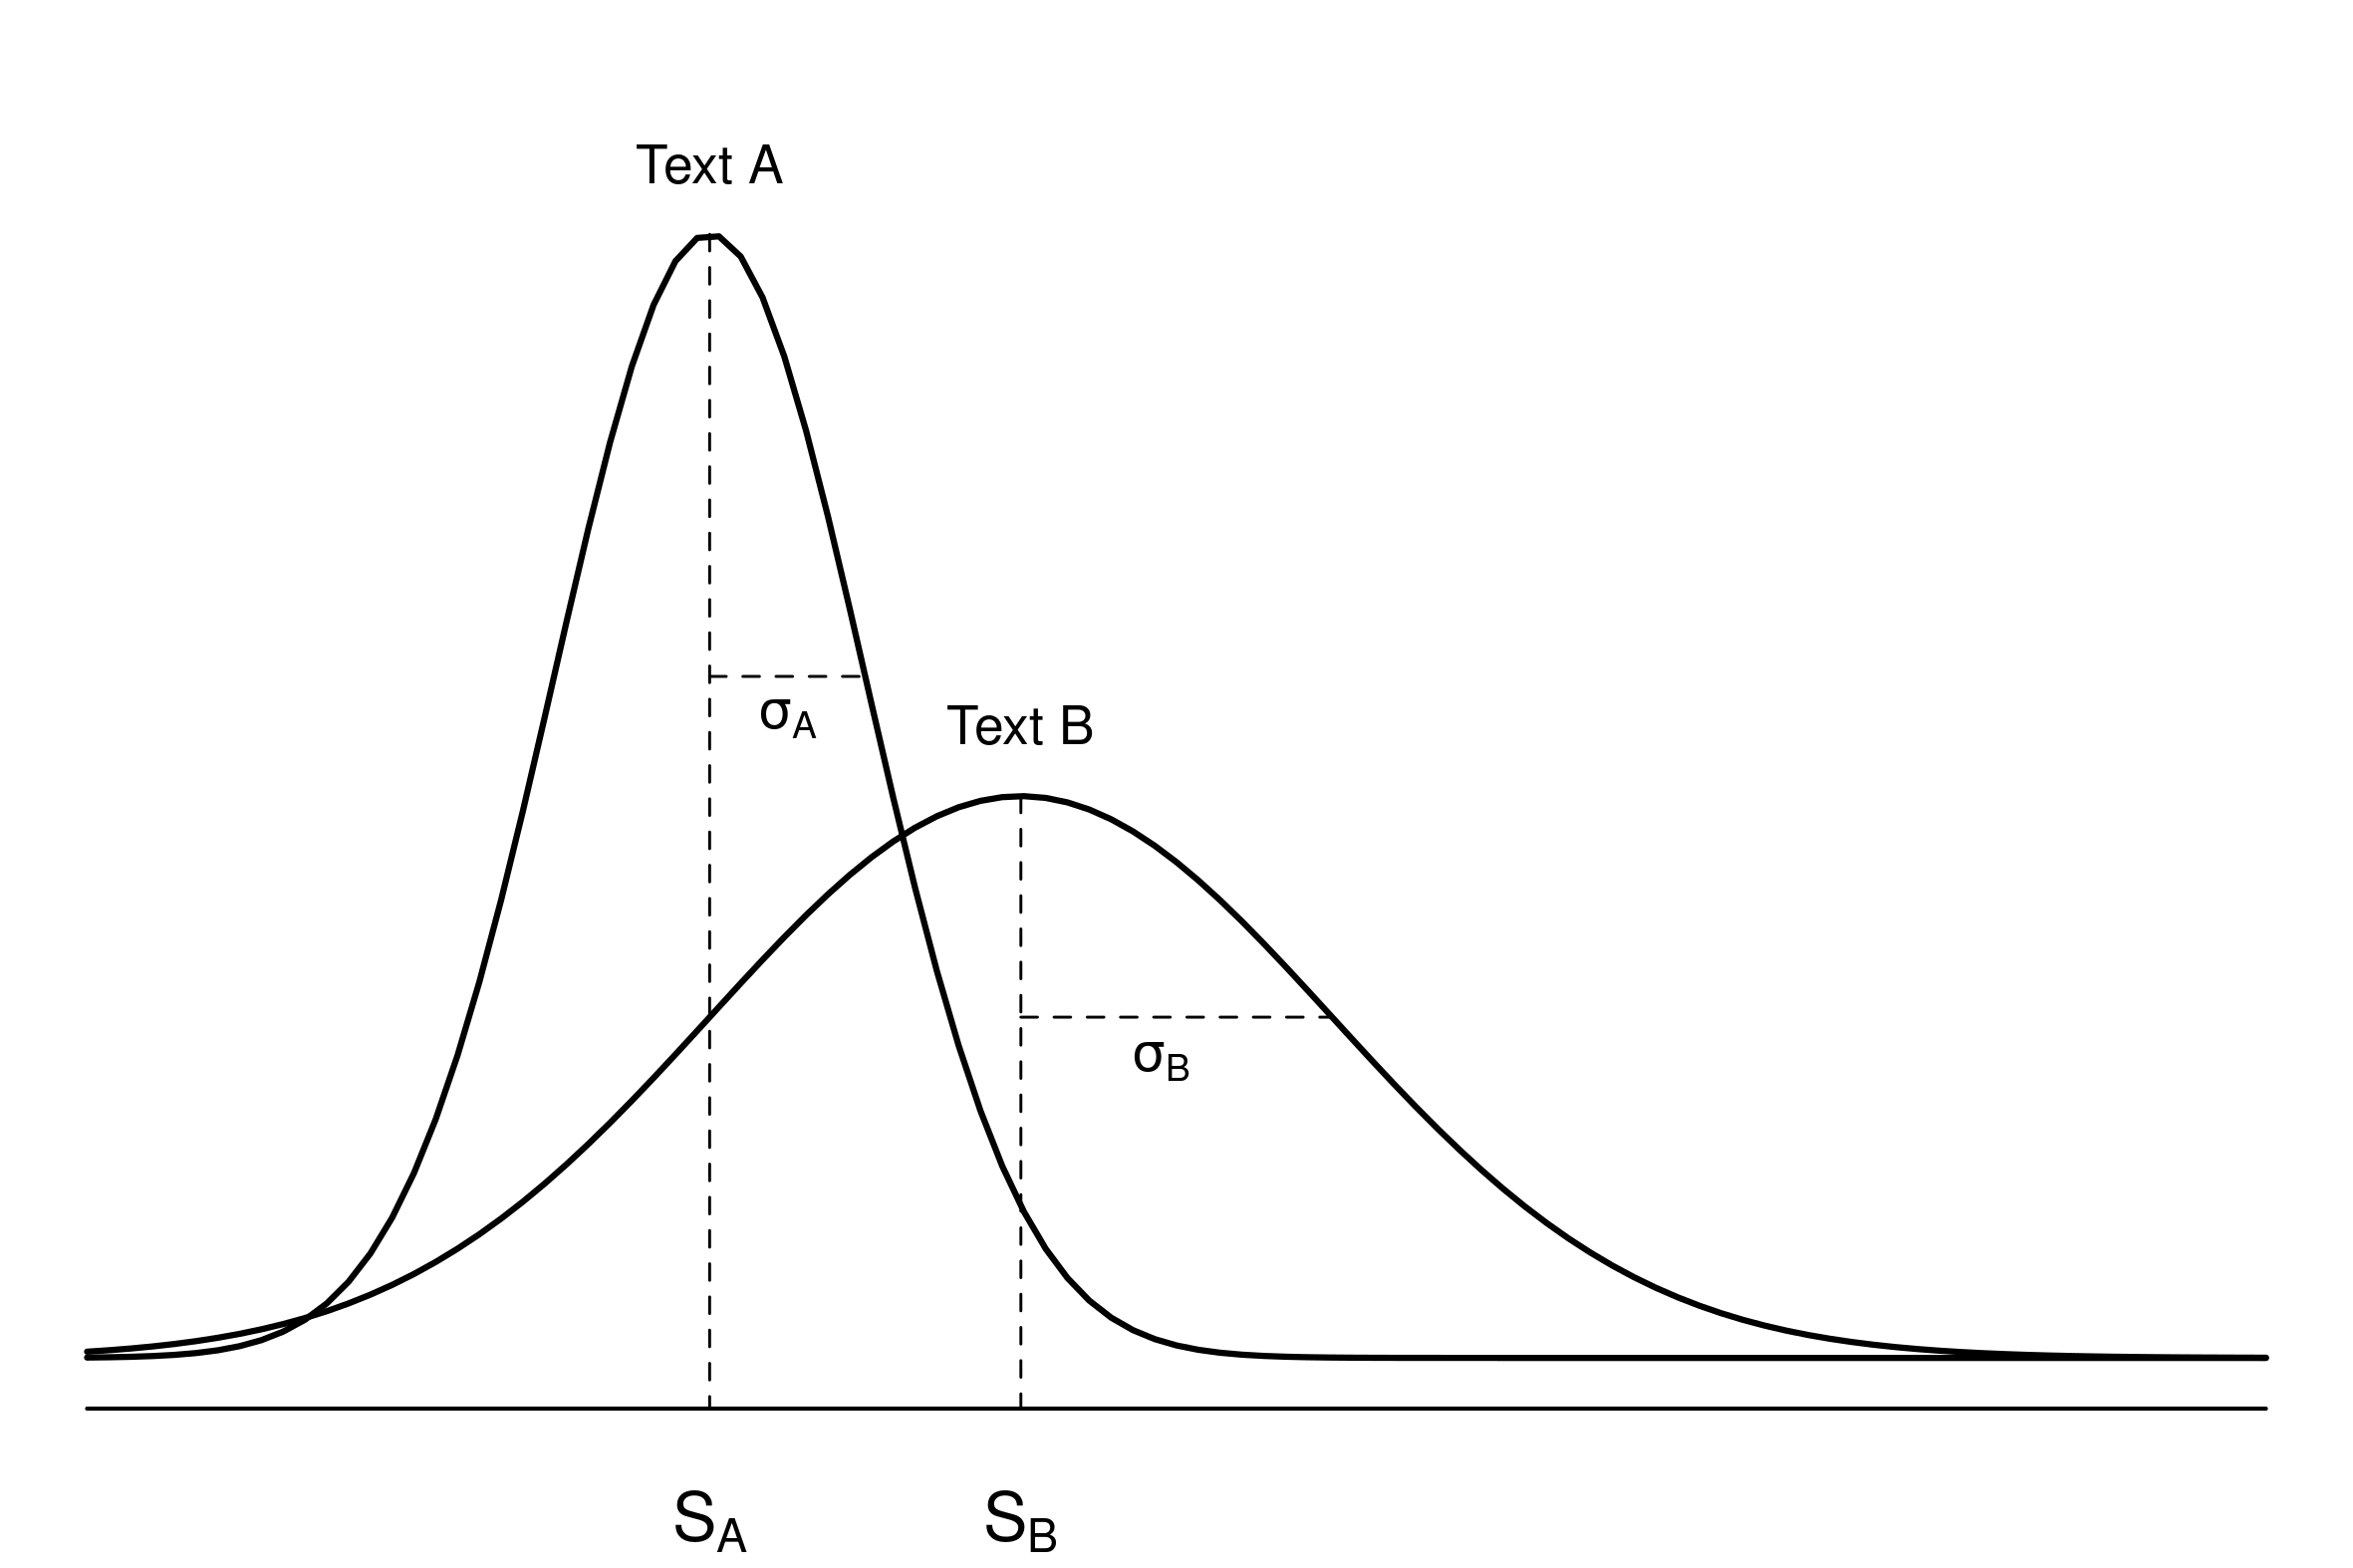
\includegraphics[width=0.7\linewidth,height=\textheight,keepaspectratio]{./images/figures/discriminal_process.png}

}

\caption{\label{fig-discriminal_process}Example distributions of the
discriminal processes for two written texts}

\end{figure}%

However, because the discriminal process of a single stimulus is not
directly observable, the theory introduces the \emph{law of comparative
judgment}. This law posits that in pairwise comparisons, a judge
perceives the stimulus positioned further along the trait continuum as
having a higher level of that trait. This principle highlights that the
outcome of a pairwise comparison likely depends on the relative distance
between stimuli rather than their absolute positions on the trait
continuum.

Thus, the theory assumes that the observed dichotomous outcome arises
from the distribution of the difference between the underlying
discriminal processes of the stimuli, known as the \emph{discriminal
difference}. Since the individual discriminal processes follow a Normal
distribution, their difference also follows a Normal distribution. The
mode (or mean) of this distribution, representing the (average) relative
separation, is given by the difference between the modal discriminal
processes of the stimuli \(S_{BA} = S_{B} - S_{A}\). Meanwhile, the
dispersion of the distribution, reflecting the variability in the
relative separation, is calculated as
\(\sigma_{BA} = \sqrt{\sigma_{B}^{2} + \sigma_{A}^{2} - \rho\sigma_{B}\sigma_{A}}\).
Here, \(\sigma_{B}\) and \(\sigma_{A}\) are the previously defined
discriminal dispersions, while \(\rho\) measures the correlation between
their discriminal processes. This correlation quantifies how much the
judge's perception of the trait in one stimulus influences his
perception of the same trait in the other.

Figure~\ref{fig-discriminal_difference} shows the distribution of the
discriminal difference for the texts depicted in
Figure~\ref{fig-discriminal_process}, assuming a correlation of
\(\rho = 0.6\). The figure reveals that, under these conditions, the
judge perceives text B as having significantly higher quality than text
A, as indicated by the shaded gray area under the curve \(P(B > A)\). As
a result, the dichotomous outcome of this comparison almost certainly
favors text B over text A.

\begin{figure}

\centering{

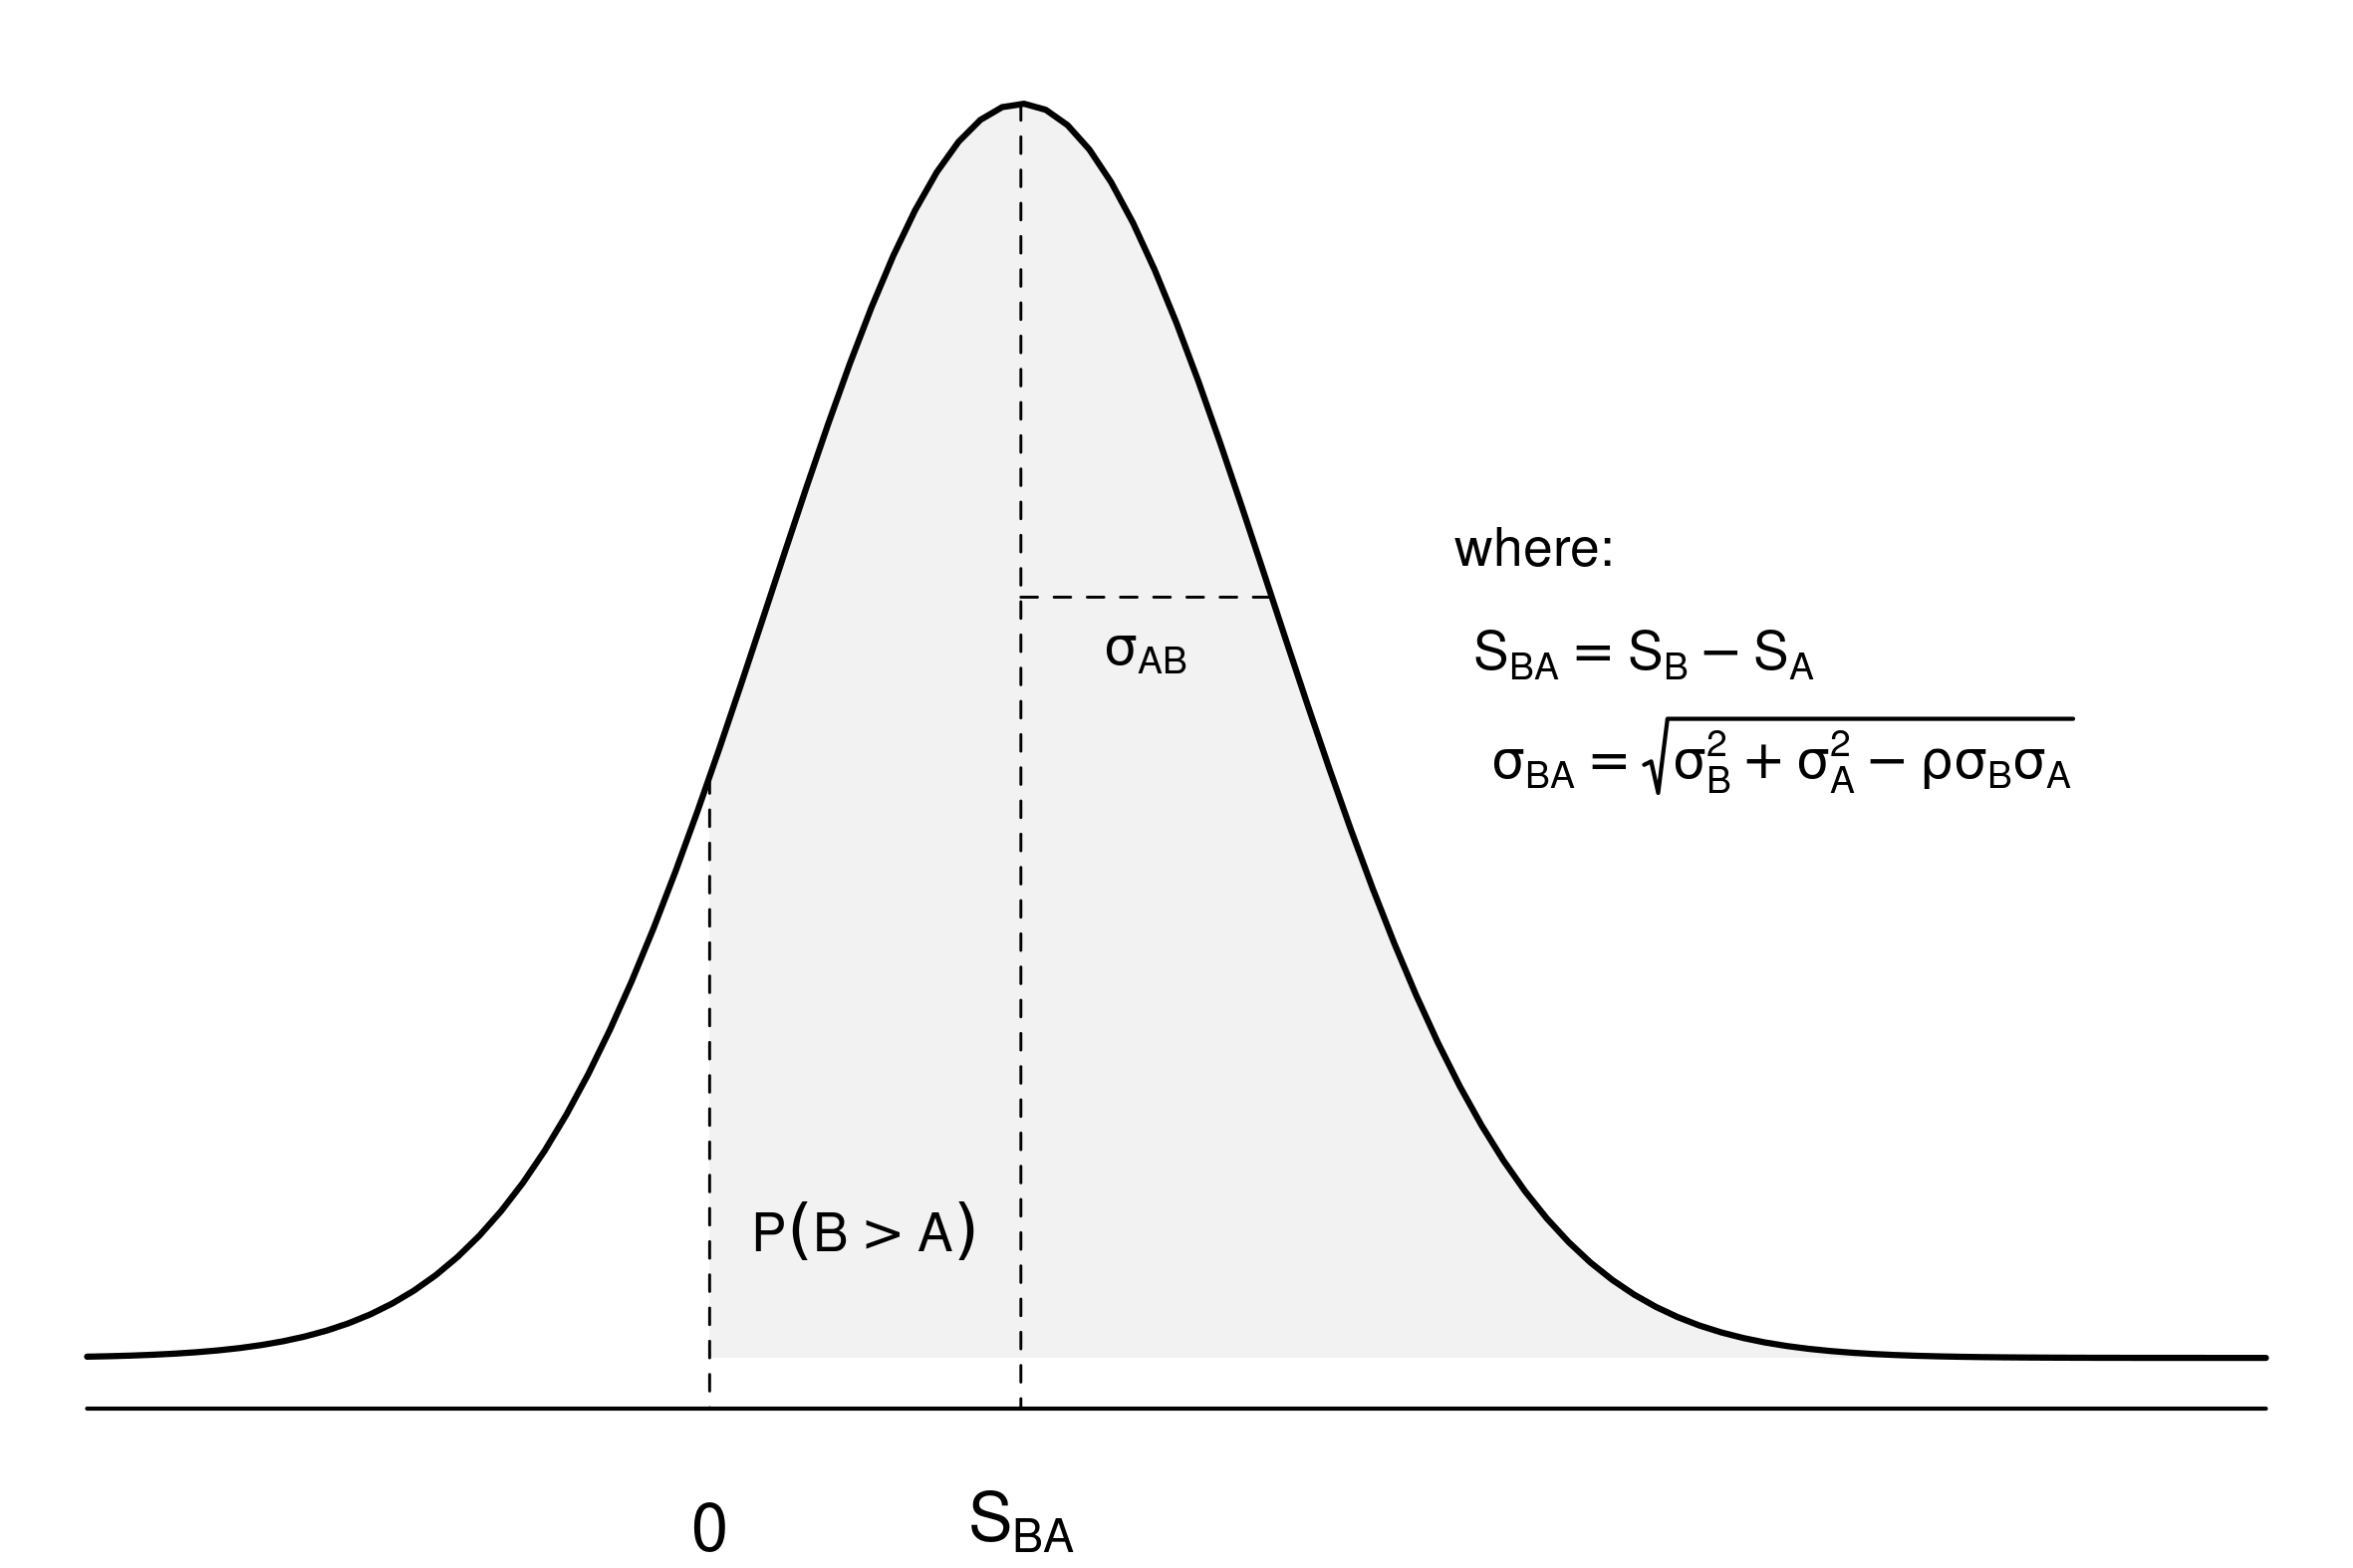
\includegraphics[width=0.7\linewidth,height=\textheight,keepaspectratio]{./images/figures/discriminal_difference.png}

}

\caption{\label{fig-discriminal_difference}Example distribution of the
discriminal difference for the two texts shown in
Figure~\ref{fig-discriminal_process}, assuming a correlation of 0.6}

\end{figure}%

Additionally, Figure~\ref{fig-correlation} illustrates how varying
correlations influence the distribution of the discriminal difference
for the same two texts. The figure shows that as the correlation
increases, indicating a stronger influence of the judge's perception of
quality in one text on his perception of the other, the distribution of
the discriminal difference becomes narrower. This narrowing affects the
area under the curve that determines the comparison outcome and,
ultimately, the conclusions drawn from this outcome.

For instance, when two texts clearly differ in quality, as depicted in
Figure~\ref{fig-discriminal_process}, higher correlations increase the
likelihood that the discriminal difference more distinctly favors text B
over text A, as indicated by the shaded gray area under the curve in
Figure~\ref{fig-correlation}. Conversely, it is easy to infer that when
the two texts have similar or identical quality levels, higher
correlations reduce the likelihood that the discriminal difference
distinctly favors one text over the other, as the distribution narrows
around zero (not depicted in the figure).

\begin{figure}

\centering{

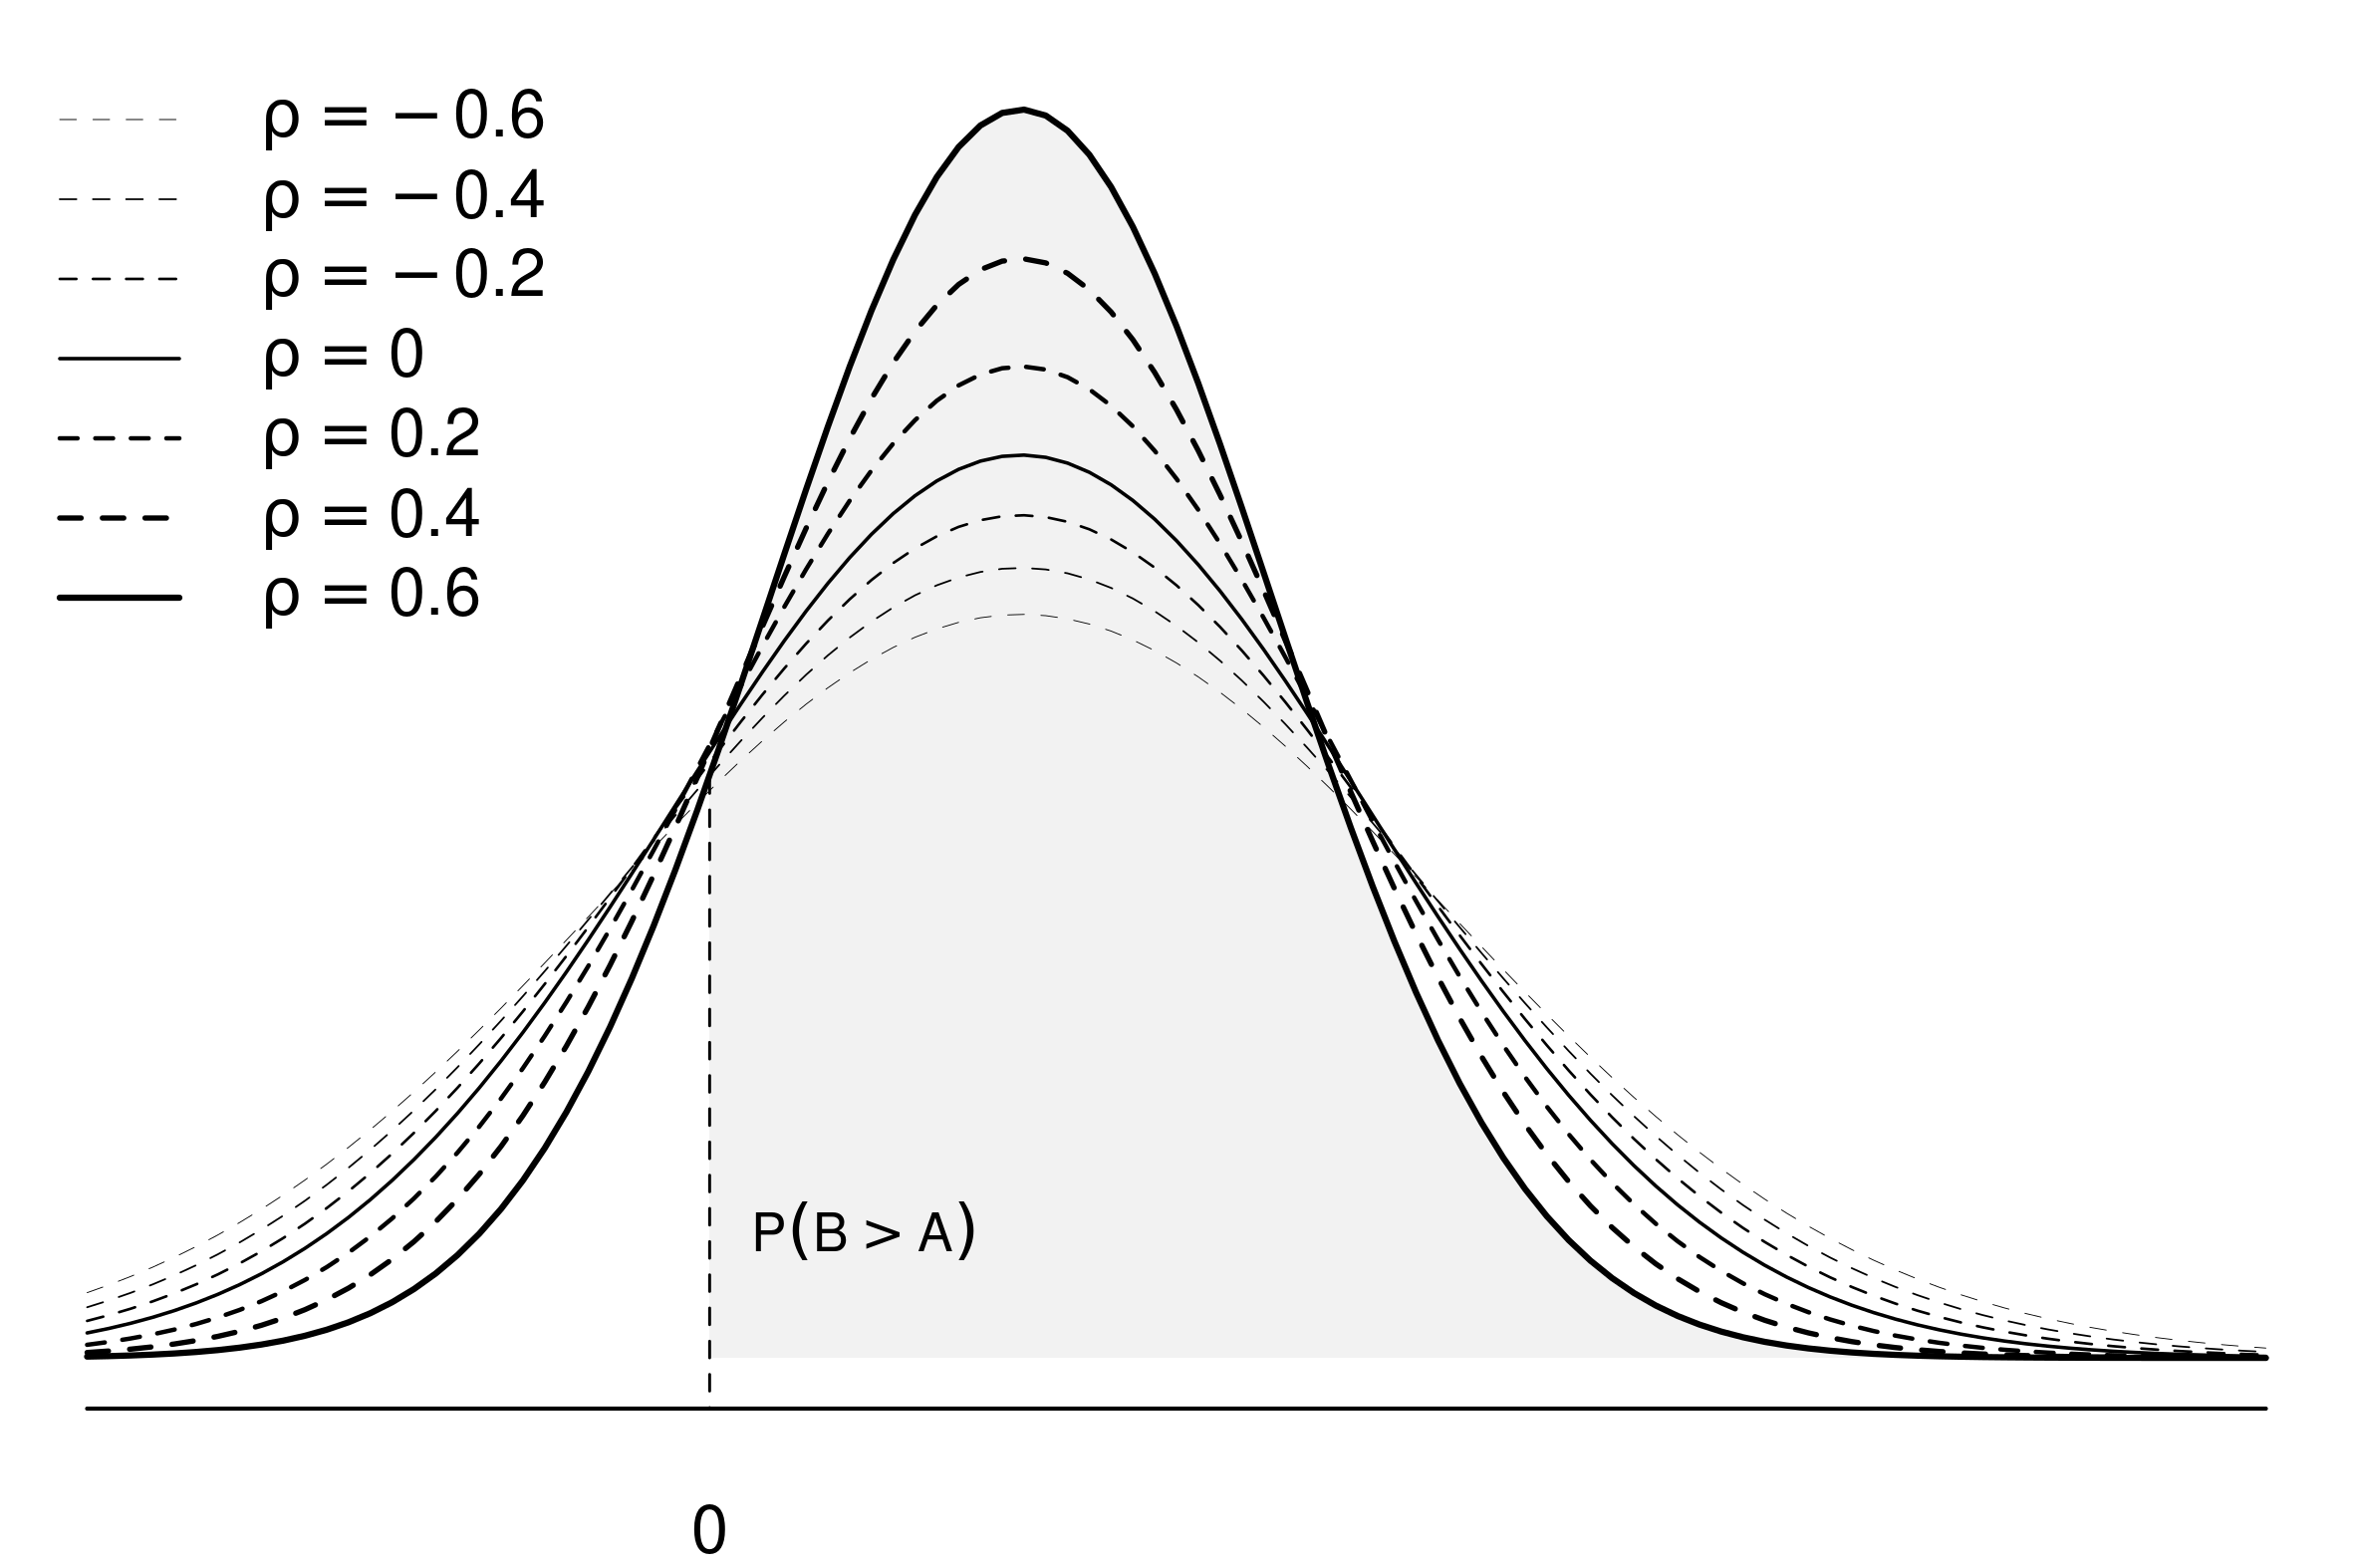
\includegraphics[width=0.7\linewidth,height=\textheight,keepaspectratio]{./images/figures/correlation.png}

}

\caption{\label{fig-correlation}The effect of correlation on the
distribution of the discriminal difference of the same two written text}

\end{figure}%

\section{Three critical issues in CJ
literature}\label{sec-theory-issues}

\subsection{The Case V and the statistical analysis of CJ
data}\label{sec-theory-issue1}

The previous section outlines the general form of Thurstone's theory,
which applies to a CJ design where a single judge evaluates multiple
stimuli. For the practical application of the theory, Thurstone
developed four additional cases derived from this general form, where
each successive case incorporates additional simplifying assumptions.
Case I represents the general form of the theory. Case II extends this
by allowing multiple judges to make comparisons rather than restricting
the comparisons to a single judge. Case III introduces the assumption of
zero correlation between stimuli. Case IV builds on this by assuming
that the stimuli have similar dispersions. Finally, Case V replaces this
assumption with the condition that the stimuli have equal discriminal
dispersions. Table~\ref{tbl-thurstone_cases} summarizes these cases and
their assumptions. For a detailed discussion of this progression, refer
to \citet{Thurstone_1927b} and \citet[pp.~248-253]{Bramley_2008}.

\begin{table}

\caption{\label{tbl-thurstone_cases}Thurstones cases and asumptions}

\centering{

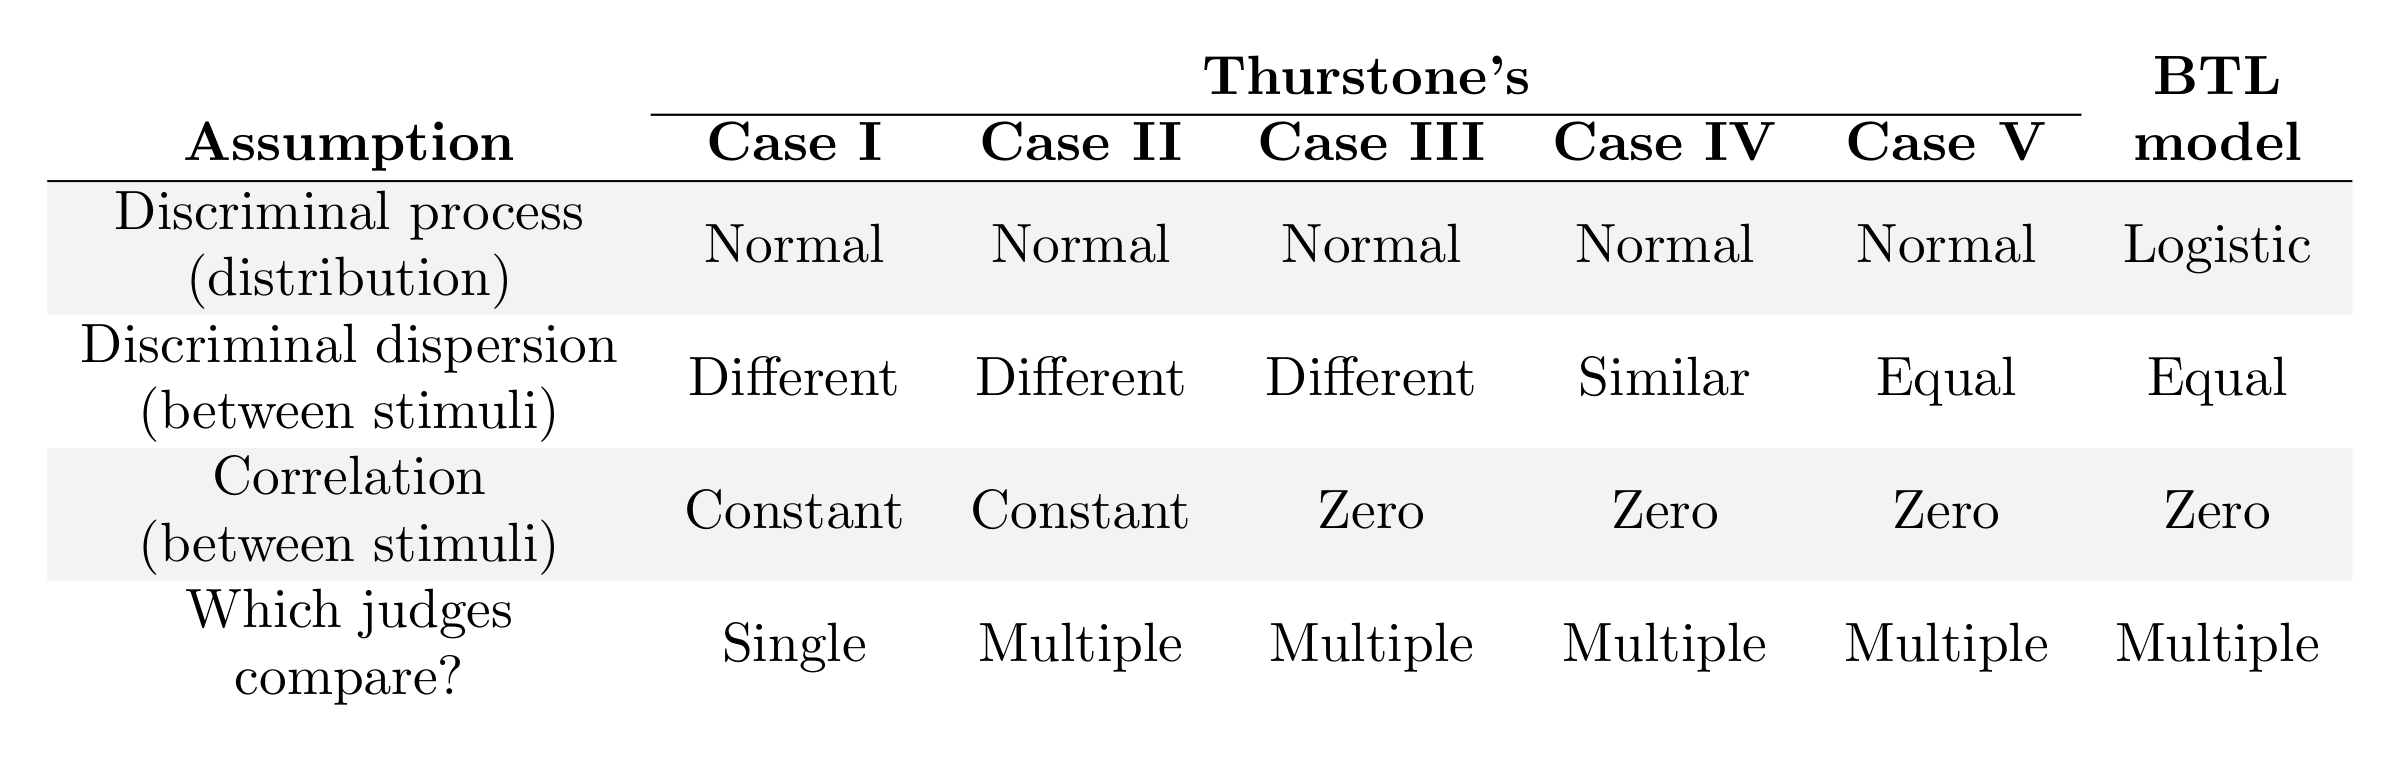
\includegraphics[width=0.9\linewidth,height=\textheight,keepaspectratio]{./images/tables/thurstone_cases.png}

}

\end{table}%

Despite its reliance on the largest number of simplifying assumptions
\citetext{\citealp[pp.~253]{Bramley_2008}; \citealp[pp.~677]{Kelly_et_al_2022}},
Case V remains the most widely used case in the CJ literature. This
popularity stems mainly from its simplified statistical representation
in the Bradley-Terry-Luce (BTL) model
\citep{Bradley_et_al_1952, Luce_1959}. The BTL model mirrors the
assumptions of Case V, with one key difference: while Case V assumes a
Normal distribution for the discriminal processes of the stimuli, the
BTL model uses the more mathematically tractable Logistic distribution
\citep[pp.~254]{Andrich_1978, Bramley_2008} (see
Table~\ref{tbl-thurstone_cases}). This substitution has little impact on
the model's estimation or interpretation, as the Normal and Logistic
distributions share similar statistical properties, differing only by a
scaling factor of approximately \(1.7\)
\citep[pp.~16]{vanderLinden_et_al_2017_I} (see
Figure~\ref{fig-logistic_vs_normal}).

\begin{figure}

\begin{minipage}{\linewidth}

\centering{

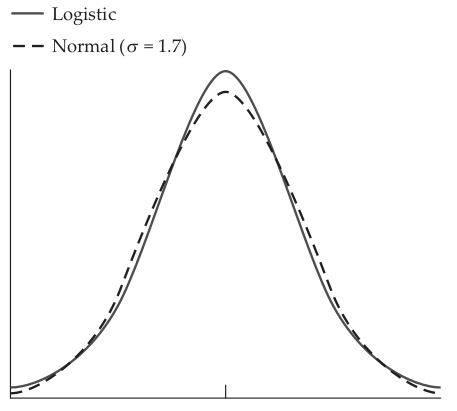
\includegraphics[width=0.7\linewidth,height=\textheight,keepaspectratio]{./images/figures/density.png}

}

\subcaption{\label{fig-density}Probability density}

\end{minipage}%
\newline
\begin{minipage}{\linewidth}

\centering{

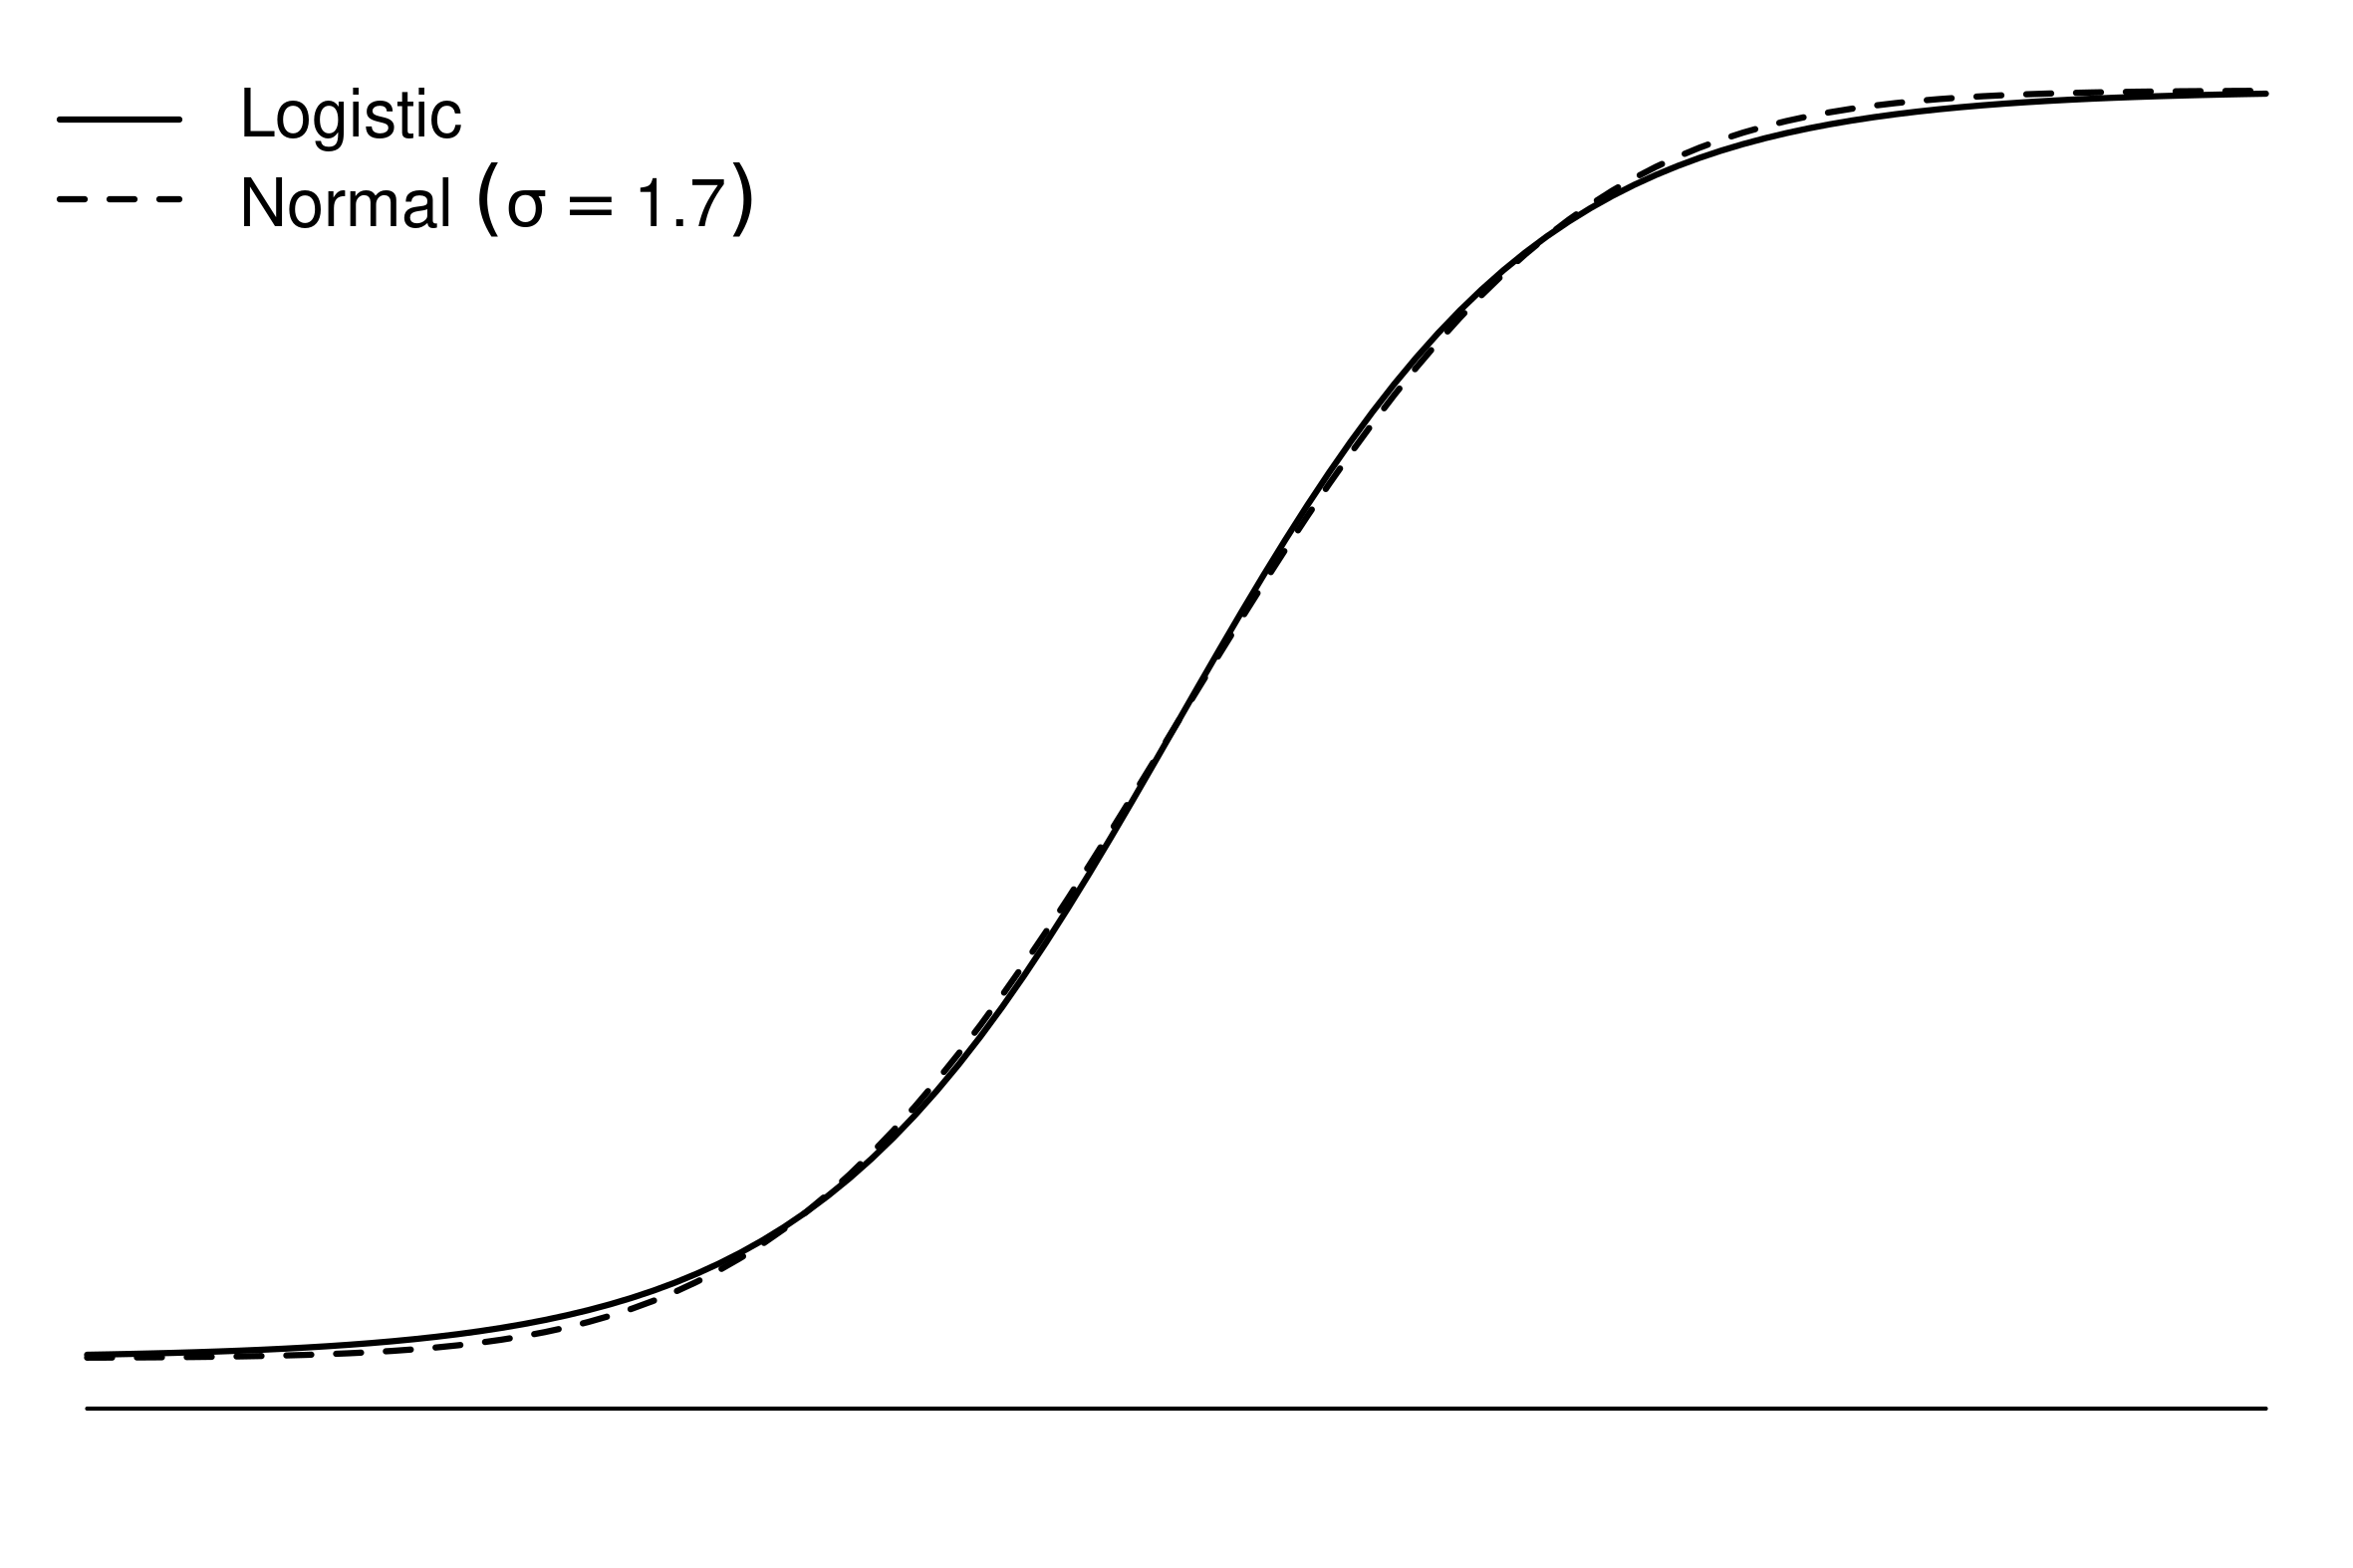
\includegraphics[width=0.7\linewidth,height=\textheight,keepaspectratio]{./images/figures/cummulative.png}

}

\subcaption{\label{fig-cumulative}Cummulative probability}

\end{minipage}%

\caption{\label{fig-logistic_vs_normal}Probability density and
cumulative probability of the logistic and Normal distributions.
Extracted from \citet[pp.~254-255]{Bramley_2008}.}

\end{figure}%

However, Thurstone originally developed Case V to provide a ``rather
coarse scaling'' of traits \citep[pp.~269]{Thurstone_1927b},
prioritizing statistical simplicity over precision in trait measurement
\citep[pp.~677]{Kelly_et_al_2022}. As a result, its assumptions may not
be suitable for applications beyond the psycho-physical contexts for
which it was created. Thurstone himself cautioned that its use ``should
not be made without (an) experimental test''
\citep[pp.~270]{Thurstone_1927b}, acknowledging that some assumptions
could prove problematic in the presence of complex traits or
heterogeneous stimuli, such as handwriting or English compositions
\citep[pp.~374]{Thurstone_1927a}. Consequently, given that modern CJ
applications frequently involve these traits and stimuli, two main
assumptions of Case V may not consistently hold in theory or practice:
the zero correlation and equal dispersion between stimuli.

As outlined in the previous section, the assumption of \emph{zero
correlation between stimuli} suggests that during a pairwise comparison,
a judge's perception of quality in one text does not influence his
perception of the same trait in another text (see
Figure~\ref{fig-correlation}, \(\rho=0\)). Thurstone attributed this
independence to the cancellation of potential judges' biases, driven by
two opposing and equally weighted effects occurring during the pairwise
comparisons \citep[pp.~268]{Thurstone_1927b}. \citet{Andrich_1978}
mathematically demonstrated this cancellation using the BTL model under
the assumption of discriminal processes with additive biases. However,
it is easy to imagine at least two scenarios where the zero correlation
assumption almost certainly does not hold: when the pairwise comparison
involves multidimensional, complex traits with heterogeneous stimuli and
when an additional hierarchical structure is relevant to the stimuli.

In the first scenario, the intricate aspects of multidimensional,
complex traits may introduce dependencies between heterogeneous stimuli
due to certain judges' biases that resist cancellation. Research on text
quality indicates that when judges evaluate these traits, they often
rely on various intricate aspects of the stimuli to form their judgments
\citep{vanDaal_et_al_2016, Lesterhuis_2018, Chambers_et_al_2022}. These
aspects, which are likely neither equally weighted nor opposing, may
influence judges' perceptions unevenly. For example, this could occur
when a judge assessing the argumentative quality of a text places
disproportionate emphasis on grammatical accuracy, ultimately favoring
texts with fewer errors but weaker arguments. Ignoring these relevant
additional ``traits'' can result in biases that resist cancellation,
introducing dependencies between stimuli
\citep[pp.~346]{vanderLinden_et_al_2017_II} and ultimately violating the
assumption of zero correlation. While direct evidence for the specific
mechanisms causing biases is lacking, studies such as
\citet{Pollitt_et_al_2003} demonstrate the presence of such biases,
supporting the idea that the factors influencing pairwise comparisons
may not always cancel out.

In the second scenario, the shared context or inherent connections
created by additional hierarchical structures may introduce dependencies
between stimuli, a statistical phenomenon commonly known as clustering
\citep{Everitt_et_al_2010}. Although the CJ literature acknowledges the
presence of such hierarchical structures in CJ data, the statistical
handling of this extra source of dependency has been inadequate. For
example, when CJ data includes multiple samples of stimuli from the same
individuals, researchers often rely on (average) estimated BTL scores to
conduct subsequent analyses and tests at the individual hierarchical
level
\citep{Bramley_et_al_2019, Boonen_et_al_2020, Bouwer_et_al_2023, vanDaal_et_al_2017, Jones_et_al_2019, Gijsen_et_al_2021}.
This approach, however, has the significant limitation of ignoring the
uncertainty associated with the BTL scores, which generates additional
statistical and measurement issues, as discussed in section
Section~\ref{sec-theory-issue2}.

In any case, the psychometric and statistical literature strongly
advises against ignoring relevant additional traits or overlooking
clustering (grouping) structures that may introduce dependencies between
stimuli. First, ignoring additional aspects pertinent to the trait of
interest can cause a dimensional mismatch, which can lead to an
overestimation of the precision (reliability) of the trait's measurement
\citep[pp.~340-341]{Hoyle_et_al_2023} or, worse, introduce bias into the
measurement process \citep{Ackerman_1989}. Additionally, overlooking
relevant hierarchical (or grouping) structures can exacerbate the
inflation of reliability by reducing the accuracy of the model's
parameters \citep[pp.~482]{Hoyle_et_al_2023}. Taken together, these
oversights undermine the reliability of the measurement process and,
since validity cannot exist without reliability
\citep[pp.~2]{Perron_et_al_2015}, ultimately compromise the validity of
the results derived from it.

\subsection{The disconnect between trait measurement and hypothesis
testing}\label{sec-theory-issue2}

Building on the previous section, it is evident that the BTL model
commonly functions as the trait's measurement model in CJ experiments
\citep{Andrich_1978, Bramley_2008}. A measurement model specifies how
manifest variables contribute to the estimation of latent variables
\citep{Everitt_et_al_2010}. For example, when evaluating text quality,
researchers use the BTL model to process the dichotomous outcomes
resulting from the pairwise comparisons (the manifest variables) to
estimate scores that reflect the underlying quality level of texts (the
latent variable)
\citep{Laming_2004, Pollitt_2012b, Whitehouse_2012, vanDaal_et_al_2016, Lesterhuis_2018_thesis, Coertjens_et_al_2017, Goossens_et_al_2018, Bouwer_et_al_2023}.

Researchers then typically use the estimated BTL scores, or their
transformations, to conduct additional analyses or hypothesis tests. For
example, these scores have been used to identify `misfit' judges and
stimuli \citep{Pollitt_2012b, vanDaal_et_al_2017, Goossens_et_al_2018},
detect biases in judges' ratings
\citep{Pollitt_et_al_2003, Pollitt_2012b}, calculate correlations with
other assessment methods \citep{Goossens_et_al_2018, Bouwer_et_al_2023},
or test hypotheses related to the underlying trait of interest
\citep{Bramley_et_al_2019, Boonen_et_al_2020, Bouwer_et_al_2023, vanDaal_et_al_2017, Jones_et_al_2019, Gijsen_et_al_2021}.

However, the statistical literature advises caution when using estimated
scores for additional analyses and tests. A key consideration is that
BTL scores are parameter estimates that inherently carry uncertainty.
Ignoring this uncertainty can bias the analysis and reduce the precision
of hypothesis tests. Notably, the direction and magnitude of such biases
are often unpredictable. Results may be attenuated, exaggerated, or
remain unaffected depending on the degree of uncertainty in the scores
and the actual effects being tested
\citetext{\citealp[pp.~25]{Kline_et_al_2023}; \citealp[pp.~137]{Hoyle_et_al_2023}}.
Finally, the reduced precision in hypothesis tests diminishes their
statistical power, increasing the likelihood of committing type-I or
type-II errors \citep{McElreath_2020}.

To mitigate these risks, principles from Structural Equation Modeling
(SEM) \citep[pp.~138]{Hoyle_et_al_2023} and Item Response Theory (IRT)
\citetext{\citealp[chap.~6]{Fox_2010}; \citealp[chap.~24]{vanderLinden_et_al_2017_I}}
recommend conducting these analyses and tests within a structural model.
A structural model specifies how different manifest or latent variables
influence the latent variable of interest \citep{Everitt_et_al_2010}.
This approach allows analyses that can account for both the BTL scores
and their uncertainties simultaneously, rather than treating them as
separate elements. Therefore, an integrated approach that combines CJ's
measurement and structural models can offer significant advantages.

\section{An updated theoretical and statistical model for
CJ}\label{sec-theory}

\subsection{The theoretical model}\label{sec-theory-theoretical}

\subsection{From theory to statistics}\label{sec-theory-statistics}

\section{Discussion}\label{sec-discuss}

\subsection{Findings}\label{sec-discuss-finding}

\subsection{Limitations and further
research}\label{sec-discuss-limitations}

\section{Conclusion}\label{sec-conclusion}

\newpage{}

\section*{Declarations}\label{declarations}
\addcontentsline{toc}{section}{Declarations}

\textbf{Funding:} The project was founded through the Research Fund of
the University of Antwerp (BOF).

\textbf{Financial interests:} The authors have no relevant financial
interest to disclose.

\textbf{Non-financial interests:} The authors have no relevant
non-financial interest to disclose.

\textbf{Ethics approval:} The University of Antwerp Research Ethics
Committee has confirmed that no ethical approval is required.

\textbf{Consent to participate:} Not applicable

\textbf{Consent for publication:} All authors have read and agreed to
the published version of the manuscript.

\textbf{Availability of data and materials:} No data was utilized in
this study.

\textbf{Code availability:} All the code utilized in this research is
available in the digital document located at:
\url{https://jriveraespejo.github.io/paper2_manuscript/}.

\textbf{AI-assisted technologies in the writing process:} The authors
used ChatGPT, an AI language model, during the preparation of this work.
They occasionally employed the tool to refine phrasing and optimize
wording, ensuring appropriate language use and enhancing the
manuscript's clarity and coherence. The authors take full responsibility
for the final content of the publication.

\textbf{CRediT authorship contribution statement:}
\emph{Conceptualization:} S.G., S.DM., T.vD., and J.M.R.E;
\emph{Methodology:} S.DM., T.vD., and J.M.R.E; \emph{Software:}
J.M.R.E.; \emph{Validation:} J.M.R.E.; \emph{Formal Analysis:} J.M.R.E.;
\emph{Investigation:} J.M.R.E; \emph{Resources:} S.G., S.DM., and T.vD.;
\emph{Data curation:} J.M.R.E.; \emph{Writing - original draft:}
J.M.R.E.; \emph{Writing - review and editing:} S.G., S.DM., and T.vD.;
\emph{Visualization:} J.M.R.E.; \emph{Supervision:} S.G. and S.DM.;
\emph{Project administration:} S.G. and S.DM.; \emph{Funding
acquisition:} S.G. and S.DM.

\newpage{}

\section*{References}\label{references}
\addcontentsline{toc}{section}{References}

\renewcommand{\bibsection}{}
\bibliography{references.bib}





\end{document}
